The picture below shows a person trying to tighten a nut with a wrench. The point of view is that of standing, facing the end of the bolt as shown and turning clockwise. Draw a free body diagram for
\begin{enumerate}
    \item The wrench only
    \item The nut only
\end{enumerate}

Then, using your FBDs, explain how the wrench is used to tighten the nut.

\begin{solution}\
\begin{center}
    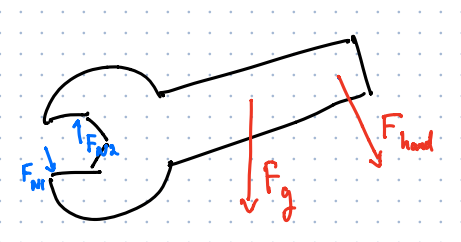
\includegraphics[width=0.75\textwidth]{img/e14p1.png}
    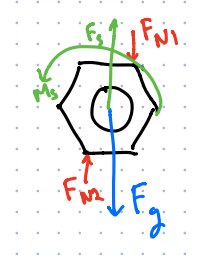
\includegraphics[width=0.5\textwidth]{img/e14p2.png}
\end{center}

The wrench transfers torque to the nuts by the normal force applied to the flat faces. If the normal force exceeds the reaction moment
\end{solution}